\documentclass[Modultest/Modultest_main.tex]{subfiles}

\begin{document}
\section{i2c\_interruptDriver}
I dette afsnit testes i2c\_interruptDriver. Testen blev foretaget efter at modultesten for boundary klassen RPI\_IF på playerside var lavet. For at se denne test refereres til dennes modultest \ref{sec:RPIIFmodultestbilag}VIRKER IKKE. Grunden til at denne klasse skulle bruges til denne test var, at for at kunne teste i2c kommunikationen var driveren nød til at have noget at sende til via i2c, og da denne klasse allerede var testet kunne den ligeså godt bruges til dette formål. Analog discovery og programmet waveforms blev også brugt. Her bruges analog discovery til at måle må kommunikationen altså SCL og SDA linjerne. I waveform kunne vi ved hjælp af logic analyzer og protocol analyzer analyserer de beskeder der bliver sendt frem og tilbage med I2C. Kommandoerne cat og echo blev brugt til henholdsvis at skrive og læse fra noderne. Da kommunikationen er ens frem og tilbage fra playerside og balldispenser blev der ikke testet med BallDispenser noden. Det første var om init(i2c\_interrupt\_init), probe(i2c\_interrupt\_probe) og open bliver kaldt, som de skal efter modulet er indsat i source tree og dtbo filen(overlay filen efter dts filen er compileret) i device tree. Nedenfor ses kernel beskederne efter init og probe.
INDSÆT BILLEDE AF INIT OG PROBE i DMESG
Open og release blev testet med et testprogram(test program ses i SOURCE CODE) vi også senere vil bruge til at teste write(i2c\_interrupt\_write) funktionen. Her vil POSIX functionerne open og close blive kaldt lige efter hinanden billedet nedefor ses kernel beskeder for dette. 
BILLEDE AF open og close
Når dette er gjort kan funktionerne for read og write testes. Først testes write, da det er den simpleste af de to, og færrest ting kunne gå galt. De første beskeder der blev sendt var state information. Alle fem "state" beskeder blev sendt. Beskederne i hex er OA(IDLE),0B (STARTING), 0C(PLAYING), 0D(LOST) og 0E(WON).  Resultatettet ses nedenfor i figur \ref{fig:states_write} i terminalen, da PSOC udskriver beskederne, hvis overførslen er succesfuld.
\begin{figure}[H]
    \centering
    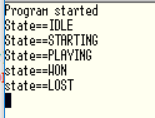
\includegraphics[width=0.5\textwidth]{Modultest/i2c_interruptDriver/graphics/states.PNG}
    \caption{Her ses de 5 "state" beskeder sendt over i2c til PSoC playerside.}
    \label{fig:states_write}
\end{figure}
Der blev også målt på denne overførsel med analog discovery et billede af dette ses i figur\ref{fig:write_analog}.
\begin{figure}[H]
    \centering
    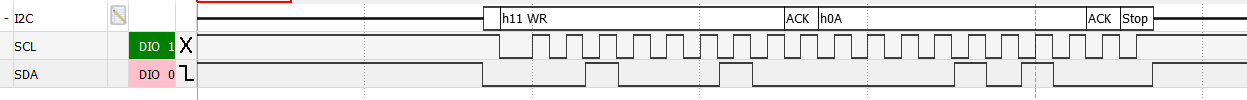
\includegraphics[width=\textwidth]{Modultest/i2c_interruptDriver/graphics/write_state_analog.PNG}
    \caption{Her vises et screenshot af beskeden med state IDLE over i2c til PSoC.}
    \label{fig:write_analog}
\end{figure}
Det næste der skulle testes var farvekoderne. Ikke alle farvekoderne blev testet, da der er for mange, så kun et par stykker blev testet. Denne overførsel består, som det også er beskrevet i arkitekturens grænsefladebeskrivelse af 5 bytes. Disse fem bytes sendt fra rtest programmet brugt til at test open og release funktionerne med. Her er den udvidet med en posix write funktion, hvor de fem bytes ligges ind i en buffer og sendes. Et eksempel på en af farvekode beskederne sendt ses i analog discovery i figur \ref{fig:write_color}.
\begin{figure}[H]
    \centering
    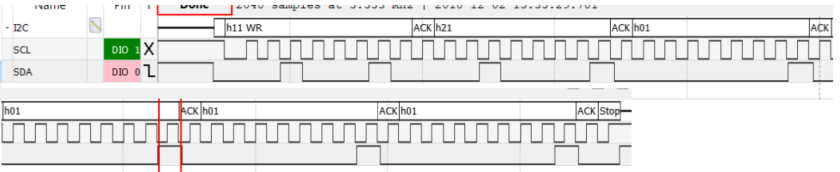
\includegraphics[width=\textwidth]{Modultest/i2c_interruptDriver/graphics/write_farvekode_analog.PNG}
    \caption{Farvekoden sendt til PSoC.}
    \label{fig:write_color}
\end{figure}
Vi kan også se resultatet i terminalen efter PSoC modtager beskeden og skriver det ud. Dette ses på figur \ref{fig:terminal_color}.
\begin{figure}[H]
    \centering
    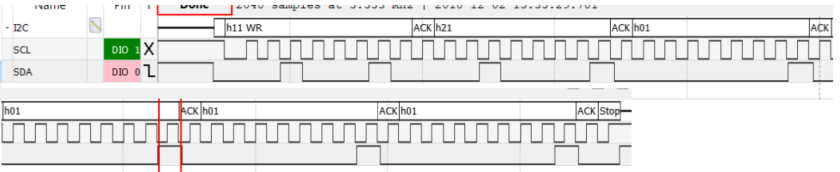
\includegraphics[width=\textwidth]{Modultest/i2c_interruptDriver/graphics/write_farvekode_analog.PNG}
    \caption{Terminal billede, hvor både modstanderen og playerside har fået skiftet farve.}
    \label{fig:terminal_color}
\end{figure}
Efter write var testet færdig blev det tid til at teste read funktionen(i2c\_interrupt\_read). Den var lidt svære at få til at virke, da der er lidt flere ting, der skal spille sammen før det virker. Kommandoen cat blev brugt, da denne kommunikation skulle testes. Da funktionen fungerer ved at når cat kaldes, så ligger funktionen sig til at sove, hvorefter et interrupt skal vække den. Det kræved altså et interrupt for at funktionen kan testes. Dette fås fra RPI\_IF klassens sendCupStatus funktion. Den sørger for at ligge noget over i dens read buffer, driveren kan læse, hvorefter den trækker interrupt benet lavt og herefter højt. Herved skabes et interrupt på driverens( og specifikke nodes) interrupt ben. Funktione ni RPI\_IF kaldes hvert sekund for denne test, så der forventes at ved at kalde cat, så vil den udskrive det den læser fra PSoC'en hvert sekund. Dette kan lade sig gøre fordi cat kommandoen konstant læser fra filen, når en positiv værdi returneres, hvilket der bliver gjort hver gang, den læser noget fra PSoC succesfuldt. Det der læses fra PSoC'en i denne test er hex værdien 3F, hvilket svarer til beskeden, der bliver sendt, når alle kopper er placeret på kopholderne. På figur \ref{fig:read_terminal} ses det i terminalen efter cat er brugt. Spørgsmålstegnet , der ses er hex værdien 3F i ascii. 
\begin{figure}[H]
    \centering
    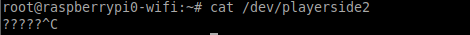
\includegraphics[width=\textwidth]{Modultest/i2c_interruptDriver/graphics/read_terminal.PNG}
    \caption{Screenshot af terminalen, hvor cat bruges til at læse fra PSoC. Spørgsmålstegnet er ascii karakteren for hex værdien 3F.}
    \label{fig:read_terminal}
\end{figure}
Der blev også lavet et screenshot af denne kommunikation i waveforms ved brug af Analog discovery. Dette ses i figur \ref{fig:read_analog}.
\begin{figure}[H]
    \centering
    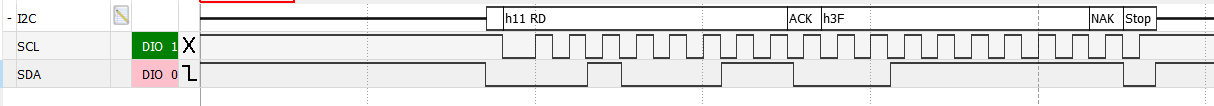
\includegraphics[width=\textwidth]{Modultest/i2c_interruptDriver/graphics/read_analog.PNG}
    \caption{Screenshot af fra waveform, hvor read kommunikationen ses.}
    \label{fig:read_analog}
\end{figure}

\end{document}